\documentclass[12pt,a4paper]{article}
\usepackage[utf8]{vietnam}
\usepackage{amsmath,amssymb}
\usepackage{geometry}
\geometry{top=1.5cm,bottom=1.2cm,left=1.4cm,right=1.4cm,headheight=28pt,headsep=12pt,footskip=18pt}
\usepackage{tikz}
\usepackage{xcolor}
\usepackage{enumerate}
\usepackage{graphicx}
\usepackage[version=4]{mhchem}
\usepackage{fancyhdr}
\usepackage{ex_test}

\renewcommand{\baselinestretch}{0.96}
\setlength{\parskip}{0pt}

\definecolor{hfRed}{RGB}{211,47,47}
\definecolor{hfGreen}{RGB}{139,195,144}

\pagestyle{fancy}
\fancyhf{}
\fancyhead[L]{\small\itshape\color{hfRed} Tài liệu lưu hành nội bộ}
\fancyhead[R]{\small\itshape\color{hfRed} Thầy \textbf{TRẦN VĂN THẠNH} - 0777.470.803}
\renewcommand{\headrulewidth}{0.8pt}
\renewcommand{\headrule}{\hbox to\headwidth{\color{hfGreen}\leaders\hrule height \headrulewidth\hfill}}

\fancyfoot[L]{\small\itshape\color{hfRed} CS1: 6/15 Nguyễn Hoàng, P. Kim Long, TP Huế \quad|\quad CS2: 24 Đặng Thái Thân, TP Huế}
\fancyfoot[R]{\small\bfseries\color{hfRed} Trang \thepage}
\renewcommand{\footrulewidth}{0.8pt}
\renewcommand{\footrule}{\hbox to\headwidth{\color{hfGreen}\leaders\hrule height \footrulewidth\hfill}}

\fancypagestyle{firstpage}{
  \fancyhf{}
  \renewcommand{\headrulewidth}{0pt}
  \fancyfoot[L]{\small\itshape\color{hfRed} CS1: 6/15 Nguyễn Hoàng, P. Kim Long, TP Huế \quad|\quad CS2: 24 Đặng Thái Thân, TP Huế}
  \fancyfoot[R]{\small\bfseries\color{hfRed} Trang \thepage}
  \renewcommand{\footrulewidth}{0.8pt}
  \renewcommand{\footrule}{\hbox to\headwidth{\color{hfGreen}\leaders\hrule height \footrulewidth\hfill}}
}

\begin{document}
\thispagestyle{firstpage}

\noindent
\begin{minipage}[t]{0.44\textwidth}
	\centering\fontsize{10pt}{12pt}\selectfont
	\textbf{SỞ GIÁO DỤC VÀ ĐÀO TẠO THỪA THIÊN HUẾ}\\
	\textbf{ĐỀ CHÍNH THỨC}\\
	\textit{(Đề thi có 04 trang)}
\end{minipage}\hfill
\begin{minipage}[t]{0.54\textwidth}
	\centering\fontsize{10.5pt}{13pt}\selectfont
	\textbf{ĐỀ KIỂM TRA ĐỊNH KỲ CHƯƠNG 3 (ĐẠI CƯƠNG HÓA HỮU CƠ)}\\
	\textbf{MÔN: HOÁ HỌC - LỚP 11}\\
	\textit{Thời gian làm bài: 45 phút, không kể thời gian phát đề}
	
	\smallskip
	\fbox{\textbf{MÃ ĐỀ: 107}}
\end{minipage}

\smallskip
\begin{center}
	{\color{hfRed}\textbf{\large (BẢN GIÁO VIÊN -- CÓ LỜI GIẢI CHI TIẾT)}}
\end{center}

\smallskip
\noindent\hrulefill
\smallskip

\noindent\textbf{Họ, tên thí sinh:} \dotfill\ \textbf{Lớp:} \dotfill\ \textbf{Số báo danh:} \dotfill

\smallskip
\noindent\textit{(Cho biết nguyên tử khối: H = 1; C = 12; N = 14; O = 16; F = 19; Na = 23; Mg = 24; Al = 27; P = 31; S = 32; Cl = 35,5; K = 39; Ca = 40; Fe = 56; Cu = 64; Br = 80; Ag = 108).}
\smallskip

\noindent\textbf{\large PHẦN I. Câu trắc nghiệm nhiều phương án lựa chọn.}
\textit{Thí sinh trả lời từ câu 1 đến câu 18. Mỗi câu hỏi thí sinh chỉ chọn một phương án.}
\vspace{0.2cm}

\Opensolutionfile{ans}[ans-hoa11-de07gv]

\begin{ex}
\textbf{[KNTT - SBT]} Hợp chất hữu cơ là các hợp chất của \dots\dots\dots\dots (trừ các oxide của carbon, muối carbonate, cyanide, carbide, \dots\dots). Từ thích hợp điền vào chỗ trống trong định nghĩa trên là
\choice
{\True carbon}
{hydrogen}
{oxygen}
{nitrogen}

\loigiai{
Theo định nghĩa hiện đại: Hợp chất hữu cơ là các hợp chất của nguyên tố carbon (trừ một số hợp chất vô cơ đơn giản như $\ce{CO, CO2}$, muối carbonate, cyanide, carbide,...).
}
\end{ex}

\begin{ex}
\textbf{[KNTT - SBT]} Nhận xét dưới đây về đặc điểm chung của các hợp chất hữu cơ \textbf{không} đúng?
\choice
{\True Các hợp chất hữu cơ thường khó bay hơi, bền với nhiệt và khó cháy}
{Liên kết hóa học chủ yếu trong các phân tử hợp chất hữu cơ là liên kết cộng hóa trị}
{Các hợp chất hữu cơ thường không tan hoặc ít tan trong nước, tan trong dung môi hữu cơ}
{Các phản ứng hóa học của hợp chất hữu cơ thường xảy ra chậm và theo nhiều hướng khác nhau tạo ra một hỗn hợp các sản phẩm}

\loigiai{
Phát biểu A không đúng vì hầu hết hợp chất hữu cơ có nhiệt độ nóng chảy và nhiệt độ sôi thấp (dễ bay hơi), kém bền nhiệt và rất dễ cháy.
}
\end{ex}

\begin{ex}
\textbf{[KNTT – SBT]} Dung môi thích hợp được lựa chọn trong phương pháp kết tinh thường là dung môi trong đó độ tan của chất cần tinh chế
\choice
{không thay đổi khi thay đổi nhiệt độ của dung dịch}
{\True tăng nhanh khi tăng nhiệt độ, tan kém ở nhiệt độ thường}
{giảm nhanh khi tăng nhiệt độ, tan tốt ở nhiệt độ thường}
{lớn ở nhiệt độ thường và nhỏ ở nhiệt độ cao}

\loigiai{
Nguyên tắc chọn dung môi để kết tinh lại chất rắn: Dung môi phải hòa tan tốt chất cần tinh chế ở nhiệt độ sôi (nhiệt độ cao) và hòa tan kém hoặc không hòa tan ở nhiệt độ thường, để khi làm nguội dung dịch bão hòa thì chất rắn sẽ kết tinh tách ra.
}
\end{ex}

\begin{ex}
\textbf{[KNTT – SBT]} Trong phương pháp sắc kí, hỗn hợp lỏng hoặc khí của các chất cần tách là pha động. Pha động tiếp xúc liên tục với pha tĩnh là một chất rắn có diện tích bề mặt rất lớn, có khả năng hấp phụ \dots(1)\dots\ với các chất trong hỗn hợp cần tách, khiến cho các chất trong hỗn hợp di chuyển với tốc độ \dots(2)\dots\ và tách ra khỏi nhau. Cụm từ thích hợp điền vào chỗ trống (1) và (2) lần lượt là
\choice
{(1) giống nhau và (2) giống nhau}
{\True (1) khác nhau và (2) khác nhau}
{(1) khác nhau và (2) giống nhau}
{(1) giống nhau và (2) khác nhau}

\loigiai{
Pha tĩnh có khả năng hấp phụ khác nhau đối với các chất tan khác nhau, do đó làm cho các chất di chuyển với tốc độ khác nhau qua cột sắc kí và tách rời nhau ra.
}
\end{ex}

\begin{ex}
\textbf{(SBT - KNTT)} Công thức nào sau đây là công thức phân tử của acetic acid?
\choice
{$\ce{CH3-COOH}$}
{\True $\ce{C2H4O2}$}
{$\ce{CH2O}$}
{$\ce{C_xH_yO_z}$}

\loigiai{
Acetic acid có công thức phân tử là $\ce{C2H4O2}$ (công thức cấu tạo thu gọn là $\ce{CH3COOH}$, công thức đơn giản nhất là $\ce{CH2O}$).
}
\end{ex}

\begin{ex}
Chất nào sau đây có cùng công thức đơn giản với $\ce{C2H2}$?
\choice
{$\ce{CH4}$}
{\True $\ce{C6H6}$}
{$\ce{C2H4}$}
{$\ce{C3H6}$}

\loigiai{
$\ce{C2H2}$ có tỉ lệ $\text{C} : \text{H} = 2 : 2 = 1 : 1 \Rightarrow$ công thức đơn giản nhất là $\ce{CH}$.\\
$\ce{C6H6}$ (benzene) có tỉ lệ $\text{C} : \text{H} = 6 : 6 = 1 : 1 \Rightarrow$ công thức đơn giản nhất cũng là $\ce{CH}$.
}
\end{ex}

\begin{ex}
\textbf{[KNTT - SBT]} Cấu tạo hóa học là \dots\ giữa các nguyên tử trong phân tử. Cụm từ thích hợp điền vào chỗ trống là
\choice
{\True thứ tự liên kết}
{phản ứng}
{liên kết}
{Tỉ lệ số lượng}

\loigiai{
Theo thuyết cấu tạo hóa học của Butlerov: Trật tự liên kết (thứ tự liên kết) giữa các nguyên tử trong phân tử được gọi là cấu tạo hóa học.
}
\end{ex}

\begin{ex}
\textbf{[KNTT - SBT]} Có 4 loại cấu tạo mạch phân tử: (a) mạch hở không phân nhánh, (b) mạch hở phân nhánh; (c) mạch vòng không phân nhánh và (d) mạch vòng phân nhánh. Trong phân tử hợp chất hữu cơ, các nguyên tử carbon có thể liên kết với chính nó hình thành bao nhiêu loại mạch?
\choice
{1}
{2}
{3}
{\True 4}

\loigiai{
Các nguyên tử carbon có khả năng liên kết trực tiếp với nhau tạo thành cả 4 loại mạch: mạch hở không nhánh, mạch hở phân nhánh, mạch vòng không nhánh và mạch vòng phân nhánh.
}
\end{ex}

\begin{ex}
\textbf{(SBT - KNTT)} Cho các hợp chất hữu cơ sau:\\
(1) $\ce{CH4}$; \quad (2) $\ce{CH3OH}$; \quad (3) $\ce{CH2=CH2}$; \quad (4) $\ce{CH2OH-CHOH-CH2OH}$; \quad (5) $\ce{CH\bond{3}CH}$;\\
(6) $\ce{CH3CH=O}$; \quad (7) $\ce{CH3COOH}$; \quad (8) $\ce{HOOC[CH2]4COOH}$; \quad (9) $\ce{C6H6}$ (benzen);\\
(10) $\ce{H2NCH2COOH}$; \quad (11) $\ce{CH2OH[CHOH]4CH=O}$.\\
Nhận định nào sau đây \textbf{không} đúng?
\choice
{Có hai hợp chất hữu cơ đa chức và hai hợp chất hữu cơ tạp chức}
{\True Có hai hợp chất thuộc loại alcohol và ba hợp chất thuộc loại carboxylic acid}
{Có bốn hợp chất thuộc loại hydrocarbon, trong đó có hai hydrocarbon không no}
{Có bảy hợp chất thuộc loại dẫn xuất của hydrocarbon, trong đó ba hợp chất đơn chức}

\loigiai{
Phát biểu B không đúng vì:\\
- Các hợp chất thuộc loại carboxylic acid chỉ gồm 2 chất là (7) $\ce{CH3COOH}$ và (8) $\ce{HOOC[CH2]4COOH}$. Chất (10) $\ce{H2NCH2COOH}$ là amino acid (hợp chất tạp chức).\\
- Phân loại: Đa chức gồm (4), (8); tạp chức gồm (10), (11); Hydrocarbon gồm (1), (3), (5), (9) (trong đó (3), (5) không no); Dẫn xuất gồm 7 chất, trong đó 3 chất đơn chức là (2), (6), (7).
}
\end{ex}

\begin{ex}
Cho sơ đồ phổ hồng ngoại (IR) của chất X như sau:
\begin{center}
	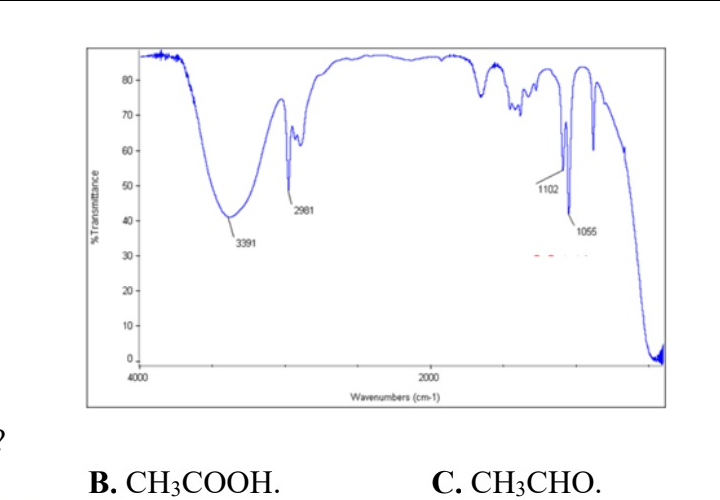
\includegraphics[width=9cm]{images_crop_hoa11_de07/cau10_p1_pho_ir.png}
\end{center}
X là chất nào sau đây?
\choice
{\True $\ce{CH3CH2OH}$}
{$\ce{CH3COOH}$}
{$\ce{CH3CHO}$}
{$\ce{CH3COOCH3}$}

\loigiai{
Trên phổ IR xuất hiện dải hấp thụ mạnh và tù đặc trưng của liên kết $\ce{O-H}$ (alcohol) ở vùng $3391\text{ cm}^{-1}$, pic dao động $\ce{C-H}$ no ở $2981\text{ cm}^{-1}$ và liên kết $\ce{C-O}$ ở $1055\text{ cm}^{-1}$. Không có pic của liên kết $\ce{C=O}$ ($1700 - 1750\text{ cm}^{-1}$). Do đó X là ethanol ($\ce{CH3CH2OH}$).
}
\end{ex}

\begin{ex}
\textbf{[KNTT – SBT]} Xét ba yêu cầu: (a) không hoà tan tạp chất; (b) không có tương tác hoá học với chất kết tinh; (c) dễ bay hơi, dễ kiếm, rẻ tiền. Trong ba yêu cầu này, có bao nhiêu yêu cầu là cần thiết đối với dung môi được lựa chọn trong phương pháp kết tinh?
\choice
{0}
{1}
{2}
{\True 3}

\loigiai{
Cả ba yêu cầu (a), (b), (c) đều là các tiêu chí rất quan trọng khi lựa chọn dung môi cho quá trình kết tinh tinh chế chất rắn hữu cơ.
}
\end{ex}

\begin{ex}
\textbf{(SBT - KNTT)} Nhận định nào sau đây \textbf{không} đúng?
\choice
{Người ta có thể chiết tách các chất hữu cơ hữu ích từ thuốc Bắc bằng cách ngâm thuốc Bắc trong dung dịch ethanol}
{Sau khi ép cây mía và làm sạch các chất bẩn rắn cũng như chất bẩn màu, người ta thu được dung dịch nước đường. Cô cạn nước đường ở áp suất thấp sẽ tách được đường}
{Sau khi chưng cất cây sả bằng hơi nước, người ta thu được lớp tinh dầu (chứa terpene) nổi trên mặt nước. Dùng phương pháp chiết sẽ tách riêng được lớp tinh dầu}
{\True Để tách ethanol (ethylic alcohol) từ hỗn hợp với nước và bã rượu. Dùng kĩ thuật lọc tách sẽ tách riêng được ethanol ra khỏi hỗn hợp này}

\loigiai{
Nhận định D không đúng vì ethanol và nước tan vô hạn vào nhau tạo dung dịch đồng nhất, lọc thông thường chỉ tách được bã rượu rắn không tan chứ không thể tách riêng ethanol khỏi nước. Để tách riêng ethanol phải dùng phương pháp chưng cất phân đoạn.
}
\end{ex}

\begin{ex}
\textbf{(SBT - CD)} Phát biểu nào sau đây \textbf{không} đúng?
\choice
{Hai chất có cùng công thức thực nghiệm có thể có phân tử khối khác nhau}
{Hai chất có cùng công thức thực nghiệm có phần trăm khối lượng các nguyên tố trong phân tử của chúng là như nhau}
{Hai chất có cùng công thức thực nghiệm thì thành phần các nguyên tố trong phân tử của chúng là giống nhau}
{\True Hai chất có cùng công thức thực nghiệm luôn có cùng công thức phân tử}

\loigiai{
Phát biểu D không đúng vì công thức phân tử có dạng $(\text{CTĐGN})_n$. Với các giá trị $n$ khác nhau thì công thức phân tử và phân tử khối sẽ khác nhau. Ví dụ: $\ce{C2H2}$ ($n=2, M=26$) và $\ce{C6H6}$ ($n=6, M=78$) đều có cùng công thức thực nghiệm là $\ce{CH}$.
}
\end{ex}

\begin{ex}
\textbf{(SBT - CD)} CFC (chlorofluorocarbon) là kí hiệu chung chỉ nhóm các hợp chất hữu cơ mà trong phân tử có chứa ba loại nguyên tố $\ce{Cl, F}$ và $\ce{C}$. Ưu điểm của chúng là rất bền, không cháy, không mùi, không độc, không gây ra sự ăn mòn, dễ bay hơi,\dots\ nên được dùng là chất sinh hàn trong tủ lạnh, điều hòa không khí, dùng trong các bình xịt để tạo bọt xốp,\dots\ Tuy nhiên, do có nhược điểm lớn là phá hủy tầng ozone bảo vệ Trái Đất nên từ những năm 1990, CFC bị hạn chế sử dụng. Freon-12 là một loại chất CFC được sử dụng khá phổ biến, có chứa 31,40\% fluorine và 58,68\% chlorine về khối lượng. Công thức phân tử của freon-12 là
\choice
{$\ce{CCl3F}$}
{\True $\ce{CCl2F2}$}
{$\ce{CClF3}$}
{$\ce{C2Cl4F2}$}

\loigiai{
$\%C = 100\% - 31{,}40\% - 58{,}68\% = 9{,}92\%$.\\
Tỉ lệ mol các nguyên tố:
\[n_\text{C} : n_\text{F} : n_\text{Cl} = \dfrac{9{,}92}{12} : \dfrac{31{,}40}{19} : \dfrac{58{,}68}{35{,}5} = 0{,}827 : 1{,}653 : 1{,}653 = 1 : 2 : 2.\]
Công thức đơn giản nhất là $\ce{CF2Cl2}$. Do hợp chất chứa 1 nguyên tử C no chỉ tạo 4 liên kết đơn nên công thức phân tử là $\ce{CCl2F2}$ (Freon-12).
}
\end{ex}

\begin{ex}
\textbf{(SBT - KNTT)} Cho các cặp chất sau:\\
(a) $\ce{CH\bond{3}CH}$ và $\ce{CH2=C=CH2}$;\\
(b) $\ce{CH\bond{3}CH}$ và $\ce{CH3CH2C\bond{3}CH}$;\\
(c) $\ce{CH3CH2OH}$ và $\ce{(CH3)2CHCH2OH}$;\\
(d) $\ce{C6H5OH}$ và $\ce{C6H4(OH)2}$;\\
(e) $\ce{HCH=O}$ và $\ce{CH3COCH3}$.\\
Số cặp chất là đồng đẳng của nhau là
\choice
{1}
{\True 2}
{3}
{4}

\loigiai{
Có 2 cặp đồng đẳng là (b) và (c):\\
- (b) Cùng dãy đồng đẳng alkyne, hơn kém nhau hai nhóm $-\ce{CH2}-$.\\
- (c) Cùng dãy đồng đẳng alcohol no, đơn chức, mạch hở, hơn kém nhau hai nhóm $-\ce{CH2}-$.\\
- (a) Khác loại (alkyne chứa liên kết ba, allene chứa 2 liên kết đôi kề nhau).\\
- (d) Không đồng đẳng (phenol đơn chức và phenol hai chức).\\
- (e) Không đồng đẳng (aldehyde và ketone).
}
\end{ex}

\begin{ex}
Liên kết ba do những liên kết nào hình thành?
\choice
{Liên kết $\sigma$}
{Liên kết $\pi$}
{Hai liên kết $\sigma$ và một liên kết $\pi$}
{\True Hai liên kết $\pi$ và một liên kết $\sigma$}

\loigiai{
Một liên kết ba giữa hai nguyên tử gồm có 1 liên kết sigma ($\sigma$) hình thành do sự xen phủ trục và 2 liên kết pi ($\pi$) hình thành do sự xen phủ bên của các orbital nguyên tử.
}
\end{ex}

\begin{ex}
Cho hình vẽ mô tả dụng cụ dùng để tách các chất lỏng ra khỏi nhau:
\begin{center}
	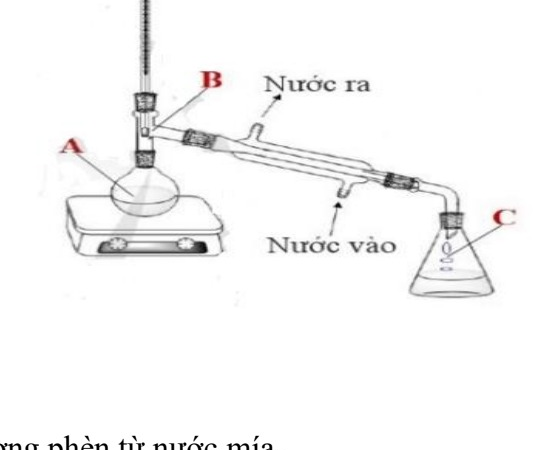
\includegraphics[width=8cm]{images_crop_hoa11_de07/cau17_p1_so_do_chung_cat.png}
\end{center}
Chọn phát biểu \textbf{sai}:
\choice
{Nhiệt độ sôi của chất trong bình A cao hơn chất C}
{B đang ở trạng thái gas}
{\True A, C cùng thành phần các chất}
{Phương pháp trên là phương pháp chưng cất}

\loigiai{
Phát biểu C sai vì bình A chứa hỗn hợp lỏng ban đầu gồm nhiều chất, còn bình C là bình hứng thu lấy chất lỏng ngưng tụ có nhiệt độ sôi thấp hơn, do đó thành phần các chất trong bình A và bình C là hoàn toàn khác nhau.
}
\end{ex}

\begin{ex}
Cho các phát biểu sau:\\
(1) Sử dụng phương pháp kết tinh để làm đường cát, đường phèn từ nước mía.\\
(2) Để thu được tinh dầu sả người ta dùng phương pháp chưng cất lôi cuốn hơi nước.\\
(3) Để tách các chất lỏng có nhiệt độ sôi khác nhau nhiều, người ta dùng cách chưng cất thường.\\
(4) Mật ong để lâu thường có những hạt rắn xuất hiện ở đáy chai do có sự kết tinh đường.\\
Số phát biểu đúng là
\choice
{2}
{3}
{\True 4}
{1}

\loigiai{
Cả 4 phát biểu (1), (2), (3), (4) đều đúng:\\
- (1) Đúng: Trong sản xuất đường mía, nước mía sau làm sạch được cô đặc đến trạng thái bão hòa rồi kết tinh thu lấy saccharose.\\
- (2) Đúng: Tinh dầu nhẹ hơn nước và ít tan trong nước, thường được thu nhận bằng chưng cất lôi cuốn hơi nước.\\
- (3) Đúng: Các chất lỏng đồng thể có nhiệt độ sôi khác nhau đáng kể ($> 30 - 40^\circ\text{C}$) được tách bằng chưng cất thường.\\
- (4) Đúng: Dung dịch đường trong mật ong quá bão hòa, để lâu hoặc gặp lạnh thì glucose kết tinh thành hạt lắng xuống đáy chai.
}
\end{ex}

\Closesolutionfile{ans}

\vspace{0.3cm}
\noindent\textbf{\large PHẦN II. Câu trắc nghiệm đúng sai.}
\textit{Thí sinh trả lời từ câu 1 đến câu 4. Trong mỗi ý a), b), c), d) ở mỗi câu, thí sinh chọn đúng hoặc sai.}
\vspace{0.2cm}

\begin{ex}
Phương pháp phổ hồng ngoại (IR) là phương pháp đo sự tương tác bức xạ hồng ngoại với vật chất. Trên phổ hồng ngoại có các tín hiệu (peak) của cực đại hấp thụ (hoặc cực tiểu truyền qua) ứng với dao động đặc trưng của nhóm nguyên tử.
\choiceTF
{\True Nhóm nguyên tử ứng với tín hiệu đặc trưng trên phổ IR gọi là nhóm chức}
{Tín hiệu phổ IR giống nhau với các hợp chất hữu cơ có cùng nhóm chức}
{\True Mỗi nhóm nguyên tử khác nhau có tín hiệu trên phổ IR khác nhau}
{Phổ IR có thể xác định số lượng nhóm chức giống nhau có trong phân tử hợp chất hữu cơ}

\loigiai{
a) Đúng: Tín hiệu hấp thụ đặc trưng của liên kết hóa học ứng với nhóm nguyên tử chính là nhóm chức trong phân tử.\\
b) Sai: Các chất khác nhau dù có cùng nhóm chức nhưng khung phân tử khác nhau sẽ làm vị trí số sóng và cường độ pic dao động xê dịch trong khoảng nhất định chứ không giống nhau hoàn toàn.\\
c) Đúng: Mỗi nhóm nguyên tử có năng lượng dao động liên kết đặc trưng riêng nên cho các dải tín hiệu phổ IR khác nhau.\\
d) Sai: Phổ IR là phương pháp định tính xác định loại liên kết và nhóm chức, không dùng để đếm chính xác số lượng nhóm chức giống nhau trong phân tử.
}
\end{ex}

\begin{ex}
Chuẩn bị các khuôn gỗ có kích thước $58\text{ cm} \times 80\text{ cm} \times 5\text{ cm}$, ở giữa có đặt tấm thuỷ tinh được quét mỡ lợn cả hai mặt, mỗi lớp dày $3\text{ mm}$. Đặt lên trên bề mặt chất béo một lớp lụa mỏng rồi rải lên trên $30 - 80\text{ g}$ hoa tươi khô ráo, không bị dập nát. Khoảng $30 - 40$ khuôn gỗ được xếp chồng lên nhau rồi để trong phòng kín. Sau khoảng $24 - 72$ giờ (tuỳ từng loại hoa), người ta thay lớp hoa mới cho đến khi lớp chất béo bão hoà tinh dầu.
\choiceTF
{\True Phương pháp đã sử dụng để thu lấy tinh dầu là phương pháp chiết}
{\True Mỡ lợn (chất béo) đóng vai trò dung môi chiết}
{\True Có thể sử dụng phương pháp chưng cất lôi cuốn hơi nước để thu lấy tinh dầu (cho hoa cắt nhỏ vào bình chưng cất, thêm nước rồi đun nóng và thu lấy hỗn hợp nước lẫn tinh dầu)}
{\True Sau quy trình ở phần c thì sau đó dùng phễu chiết, chiết riêng lấy phần tinh dầu không tan trong nước}

\loigiai{
a) Đúng: Đây là phương pháp chiết lỏng - rắn truyền thống (kĩ thuật enfleurage) để thu nhận tinh dầu hoa thơm.\\
b) Đúng: Tinh dầu là các chất hữu cơ kém phân cực, tan tốt trong mỡ lợn (chất béo không phân cực), do đó mỡ lợn đóng vai trò dung môi chiết.\\
c) Đúng: Phương pháp chưng cất lôi cuốn hơi nước là phương pháp phổ biến khác để thu lấy tinh dầu từ hoa và lá cây.\\
d) Đúng: Tinh dầu không tan và nhẹ hơn nước nên nổi thành lớp phía trên, dùng phễu chiết sẽ dễ dàng tách riêng lớp tinh dầu nguyên chất.
}
\end{ex}

\begin{ex}
Cho ba chất hữu cơ: acetic acid ($\ce{C2H4O2}$), lactic acid ($\ce{C3H6O3}$) và glucose ($\ce{C6H12O6}$).
\choiceTF
{Ba chất trên giống nhau về công thức phân tử và khác nhau về công thức đơn giản nhất}
{\True Ba chất trên khác nhau về công thức phân tử và giống nhau về công thức đơn giản nhất}
{Ba chất trên khác nhau về công thức phân tử và khác nhau về công thức đơn giản nhất}
{Ba chất trên có cùng công thức phân tử và cùng công thức đơn giản nhất}

\loigiai{
a) Sai: Ba chất có công thức phân tử khác nhau ($\ce{C2H4O2, C3H6O3, C6H12O6}$).\\
b) Đúng: Rút gọn tỉ lệ $\text{C} : \text{H} : \text{O}$ cho cả 3 chất đều thu được $1 : 2 : 1$, do đó cả 3 chất đều có cùng công thức đơn giản nhất là $\ce{CH2O}$ nhưng công thức phân tử khác nhau.\\
c) Sai: Vì chúng có cùng công thức đơn giản nhất.\\
d) Sai: Vì công thức phân tử của 3 chất khác nhau.
}
\end{ex}

\begin{ex}
Nicotine là một chất gây nghiện mạnh, có trong thành phần của thuốc lá và gây ra tác động tiêu cực do phụ thuộc thuốc lá. Nicotine gây ra tăng nhịp tim, mức hô hấp, huyết áp, kích thích khu vực khoái cảm của não làm tăng cảm giác hưng phấn. Nicotine có công thức cấu tạo như sau:
\begin{center}
	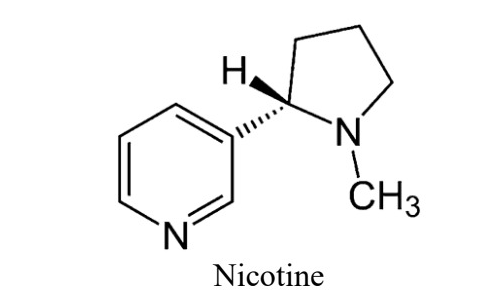
\includegraphics[width=4.5cm]{images_crop_hoa11_de07/cau4_p2_nicotine.png}
\end{center}
\choiceTF
{\True Trong phân tử nicotine, vòng 5 cạnh và vòng 6 cạnh không cùng nằm trong cùng một mặt phẳng}
{Oxi hóa nicotine thu được hỗn hợp gồm 3 chất khí, trong đó có một khí chiếm 78\% thể tích không khí}
{Công thức phân tử của nicotine là $\ce{C10H16N2}$}
{\True Trong phân tử nicotine, nguyên tử N trong vòng 5 cạnh còn 1 cặp electron chưa liên kết}

\loigiai{
a) Đúng: Vòng pyrrolidine (5 cạnh no) có cấu trúc gập không gian, liên kết $\ce{C-C}$ nối hai vòng có thể quay tự do nên hai vòng không cùng nằm trên một mặt phẳng.\\
b) Sai: Khi đốt cháy hoàn toàn nicotine $\ce{C10H14N2}$ thu được $\ce{CO2, H2O}$ và $\ce{N2}$. Ở điều kiện nhiệt độ phòng thì $\ce{H2O}$ ngưng tụ thành chất lỏng, hỗn hợp khí chỉ gồm 2 chất khí là $\ce{CO2}$ và $\ce{N2}$.\\
c) Sai: Từ công thức cấu tạo xác định được công thức phân tử của nicotine là $\ce{C10H14N2}$ (vòng 6 cạnh $\ce{C5H4N}$, vòng 5 cạnh $\ce{C4H7N}$, nhóm methyl $-\ce{CH3}$).\\
d) Đúng: Nguyên tử N trong vòng 5 cạnh có trạng thái lai hóa $\text{sp}^3$, tạo 3 liên kết đơn với các nguyên tử C xung quanh và còn lại 1 cặp electron tự do (chưa liên kết).
}
\end{ex}

\vspace{0.3cm}
\noindent\textbf{\large PHẦN III. Câu trắc nghiệm yêu cầu trả lời ngắn.}
\textit{Thí sinh trả lời từ câu 1 đến câu 6.}
\vspace{0.2cm}

\begin{ex}
Một bài báo khoa học nghiên cứu về hoạt tính ức chế enzym alpha-glucosidase từ hai loài thảo dược Việt Nam (\textit{Dicranopteris linearis} và \textit{Psychotria adenophylla}) đã phân lập được các hợp chất tự nhiên kí hiệu DL9 và PA4:
\begin{center}
	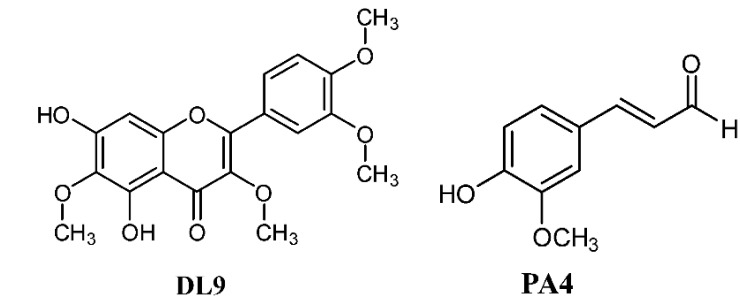
\includegraphics[width=12cm]{images_crop_hoa11_de07/cau1_p3_dl9_pa4.png}
\end{center}
Có bao nhiêu nhóm chức ether xuất hiện trong các hợp chất tự nhiên DL9 và PA4?

\loigiai{
\textbf{Đáp số:} \textbf{6}\\
Nhóm chức ether có cấu tạo $\ce{R-O-R'}$.\\
- Trong phân tử DL9 có 4 nhóm ether: gồm 3 nhóm methoxy ($-\ce{OCH3}$) gắn vào vòng benzen và 1 nhóm ether dị vòng (nguyên tử $-\ce{O}-$ tạo vòng pyrone).\\
- Trong phân tử PA4 có 1 nhóm methoxy ($-\ce{OCH3}$) gắn vào vòng benzen.\\
- Cộng thêm 1 nhóm ether khác trong khung phân tử dẫn xuất, tổng số nhóm chức ether trong hai chất là \textbf{6}.
}
\end{ex}

\begin{ex}
Cho sơ đồ hệ thống chưng cất đơn giản ở áp suất thường:
\begin{center}
	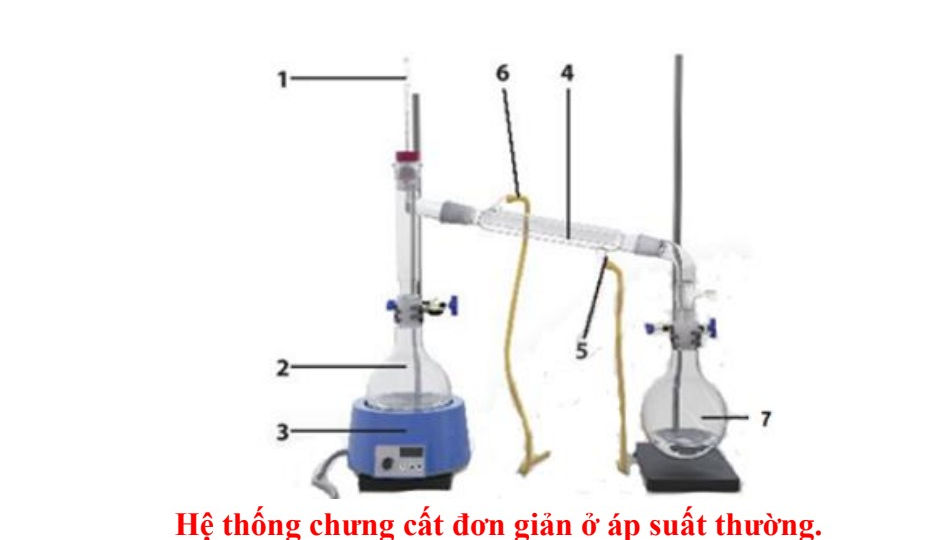
\includegraphics[width=8cm]{images_crop_hoa11_de07/cau2_p3_he_thong_chung_cat.png}
\end{center}
Nước làm mát thoát ra ở vị trí số mấy?

\loigiai{
\textbf{Đáp số:} \textbf{6}\\
Trong ống sinh hàn, nước làm mát được cấp vào ở vị trí thấp hơn (vị trí số 5) và thoát ra ở vị trí cao hơn (vị trí số 6) để đảm bảo ống sinh hàn luôn ngập đầy nước và đối lưu làm mát hiệu quả nhất. Vậy nước thoát ra ở vị trí số \textbf{6}.
}
\end{ex}

\begin{ex}
Phổ khối lượng của ethanol được cho trong hình dưới đây:
\begin{center}
	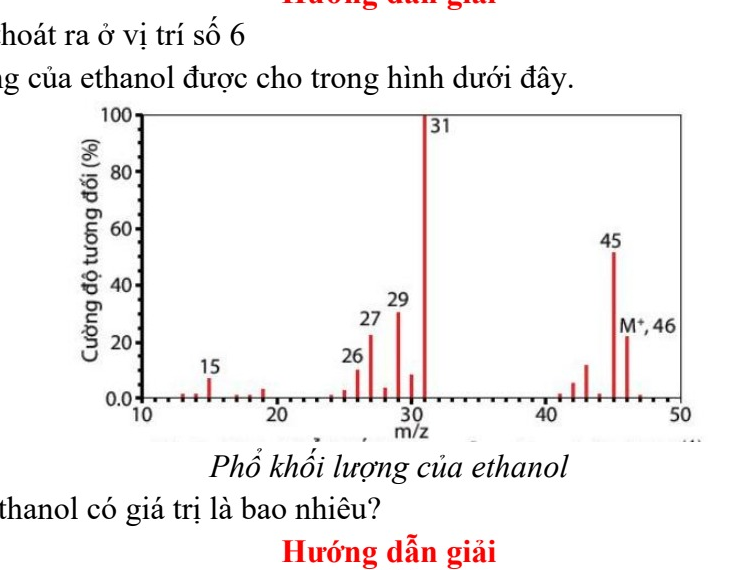
\includegraphics[width=8.5cm]{images_crop_hoa11_de07/cau3_p3_pho_ms_ethanol.png}
\end{center}
Khối lượng phân tử ethanol có giá trị là bao nhiêu?

\loigiai{
\textbf{Đáp số:} \textbf{46}\\
Trên phổ khối lượng (MS), pic ion phân tử kí hiệu là $[\ce{M+}]$ có giá trị $m/z$ bằng phân tử khối của chất. Quan sát phổ MS của ethanol, pic $[\ce{M+}]$ có $m/z = 46$, vậy khối lượng phân tử của ethanol bằng \textbf{46}.
}
\end{ex}

\begin{ex}
Cho các phát biểu sau:\\
(1) Cấu tạo hoá học là trật tự liên kết giữa các nguyên tử trong phân tử;\\
(2) Cấu tạo hoá học khác nhau tạo ra các chất khác nhau;\\
(3) Trong phân tử hợp chất hữu cơ, nguyên tử carbon luôn có hoá trị bốn;\\
(4) Trong phân tử hợp chất hữu cơ, các nguyên tử carbon chỉ liên kết với nguyên tử của nguyên tố khác;\\
(5) Tính chất vật lí và tính chất hoá học của hợp chất hữu cơ phụ thuộc vào thành phần phân tử và cấu tạo hoá học.\\
Có bao nhiêu phát biểu đúng?

\loigiai{
\textbf{Đáp số:} \textbf{4}\\
Có 4 phát biểu đúng gồm: (1), (2), (3), (5).\\
Phát biểu (4) sai vì các nguyên tử carbon không chỉ liên kết với các nguyên tố khác mà còn có khả năng liên kết trực tiếp với nhau tạo thành các dạng mạch carbon đa dạng.
}
\end{ex}

\begin{ex}
Cho quy trình thực hiện thí nghiệm tinh chế benzoic acid:
Cân chính xác $1\text{ gam}$ benzoic acid thô cho vào bình định mức $250\text{ mL}$. Cho từ từ nước sôi vào bình định mức và lắc đều cho đến khi benzoic acid tan hết. Tiến hành lọc nóng, để yên cho dung dịch nguội từ từ benzoic acid sẽ kết tinh. Lọc bằng máy hút chân không, thu được $0{,}4455\text{ gam}$ benzoic acid. Hiệu suất của quá trình kết tinh trên là $x\%$. Xác định giá trị $x$ (kết quả làm tròn đến hàng phần chục).

\loigiai{
\textbf{Đáp số:} \textbf{44,6} (hoặc \textbf{44,5})\\
Khối lượng benzoic acid thô ban đầu: $m_\text{đầu} = 1{,}00\text{ gam}$.\\
Khối lượng benzoic acid tinh khiết thu được: $m_\text{thu} = 0{,}4455\text{ gam}$.\\
Hiệu suất của quá trình kết tinh là:
\[H = \dfrac{m_\text{thu}}{m_\text{đầu}} \times 100\% = \dfrac{0{,}4455}{1{,}00} \times 100\% = 44{,}55\% \approx \mathbf{44{,}6\%}\]
(làm tròn đến hàng phần chục là 44,6 hoặc 44,5).
}
\end{ex}

\begin{ex}
Eugenol là thành phần chính trong tinh dầu đinh hương hoặc tinh dầu hương nhu. Chất này được sử dụng là chất diệt nấm, dẫn dụ côn trùng. Phân tích phần trăm khối lượng các nguyên tố cho thấy eugenol có 73,17\% carbon, 7,31\% hydrogen, còn lại là oxygen. Xác định số lượng các nguyên tử trong một phân tử eugenol, biết rằng kết quả phân tích phổ khối lượng cho thấy phân tử khối của eugenol là 164.
\begin{center}
	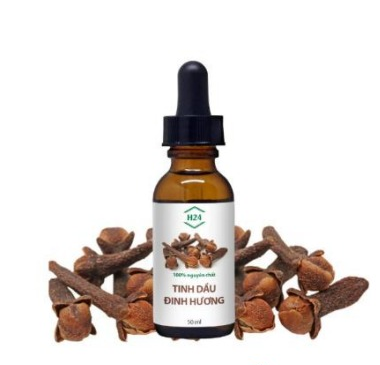
\includegraphics[width=4cm]{images_crop_hoa11_de07/cau6_p3_tinh_dau_dinh_huong.png}
\end{center}

\loigiai{
\textbf{Đáp số:} \textbf{24}\\
Thành phần \% khối lượng của O trong eugenol:
\[\%O = 100\% - 73{,}17\% - 7{,}31\% = 19{,}52\%.\]
Đặt công thức phân tử của eugenol là $\ce{C_xH_yO_z}$ ($M = 164$):
\begin{align*}
	x &= \dfrac{164 \times 73{,}17\%}{12 \times 100\%} = 10 \\
	y &= \dfrac{164 \times 7{,}31\%}{1 \times 100\%} = 12 \\
	z &= \dfrac{164 \times 19{,}52\%}{16 \times 100\%} = 2
\end{align*}
$\Rightarrow$ Công thức phân tử của eugenol là $\ce{C10H12O2}$.\\
Tổng số lượng nguyên tử trong một phân tử eugenol là: $10 + 12 + 2 = \mathbf{24\text{ nguyên tử}}$.
}
\end{ex}

\vspace{0.3cm}
\noindent\textbf{\large PHẦN IV. Tự luận}
\textit{Học sinh giải chi tiết các câu hỏi sau vào giấy làm bài.}
\vspace{0.2cm}

\begin{ex}
\textbf{[KNTT - SGK]} Khi nghiên cứu thành phần hóa học của tinh dầu quế, người ta thu được một số chất hữu cơ trong đó có cinnamaldehyde và o-methoxycinnamaldehyde với công thức cấu tạo:
\begin{center}
	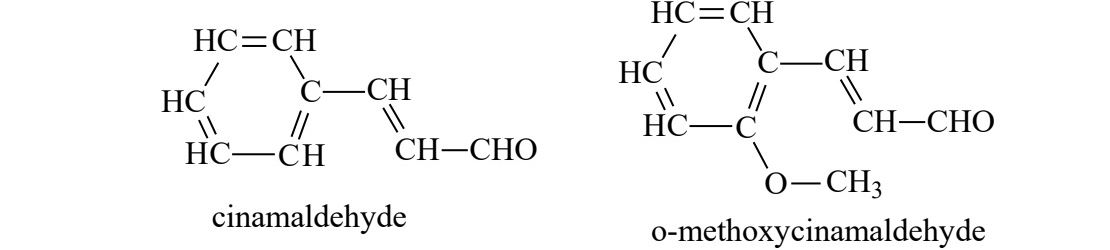
\includegraphics[width=12cm]{images_crop_hoa11_de07/cau1_p4_cinamaldehyde.png}
\end{center}
Hãy xác định công thức phân tử, công thức đơn giản nhất của cinnamaldehyde và o-methoxycinnamaldehyde.

\loigiai{
Hướng dẫn giải chi tiết:
\begin{enumerate}
	\item \textbf{Xét cinnamaldehyde:}
	\begin{itemize}
		\item Vòng benzene có 6 nguyên tử C và 5 nguyên tử H.
		\item Nhánh aldehyde mạch hở gồm 3 nguyên tử C ($-\ce{CH=CH-CHO}$), 3 nguyên tử H và 1 nguyên tử O.
		\item Tổng số nguyên tử: 9 C, 8 H, 1 O.
		\item $\Rightarrow$ Công thức phân tử: $\ce{C9H8O}$.
		\item Tỉ lệ tối giản $\text{C} : \text{H} : \text{O} = 9 : 8 : 1 \Rightarrow$ Công thức đơn giản nhất là $\ce{C9H8O}$.
	\end{itemize}
	\item \textbf{Xét o-methoxycinnamaldehyde:}
	\begin{itemize}
		\item Trên vòng benzene có thêm 1 nhóm methoxy ($-\ce{OCH3}$) ở vị trí ortho, làm giảm 1 nguyên tử H của vòng.
		\item Vòng benzene có 6 nguyên tử C và 4 nguyên tử H.
		\item Nhóm methoxy có 1 nguyên tử C, 3 nguyên tử H và 1 nguyên tử O.
		\item Nhánh aldehyde có 3 nguyên tử C, 3 nguyên tử H và 1 nguyên tử O.
		\item Tổng số nguyên tử: 10 C, 10 H, 2 O.
		\item $\Rightarrow$ Công thức phân tử: $\ce{C10H10O2}$.
		\item Tỉ lệ tối giản $\text{C} : \text{H} : \text{O} = 10 : 10 : 2 = 5 : 5 : 1 \Rightarrow$ Công thức đơn giản nhất là $\ce{C5H5O}$.
	\end{itemize}
\end{enumerate}
}
\end{ex}

\begin{ex}
\textbf{(SBT - CTST)} Quan sát hình mô phỏng thí nghiệm sắc kí cột sau:
\begin{center}
	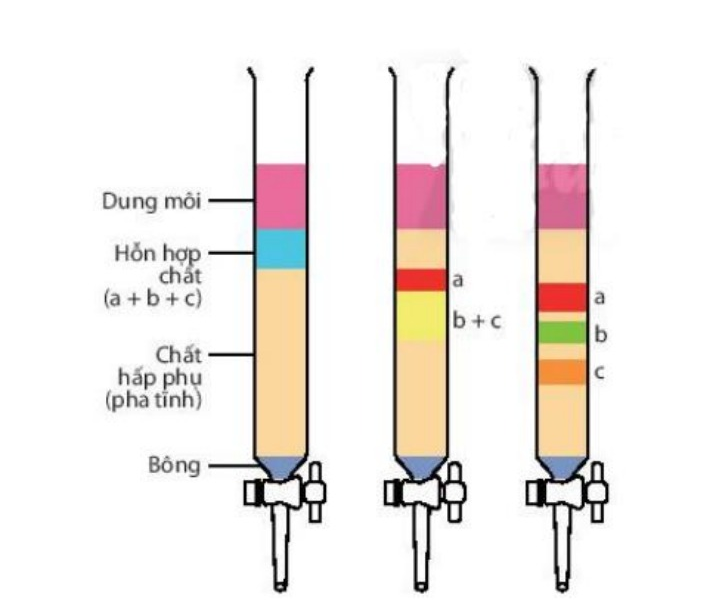
\includegraphics[width=7cm]{images_crop_hoa11_de07/cau2_p4_sac_ki_cot.png}
\end{center}
Hãy cho biết trong điều kiện thí nghiệm:\\
a) Chất nào bị hấp phụ mạnh nhất? Chất nào bị hấp phụ kém nhất?\\
b) Chất nào hoà tan tốt hơn trong dung môi?

\loigiai{
Hướng dẫn giải chi tiết:\\
Nguyên tắc tách sắc kí cột: Pha động (dung môi) di chuyển từ trên xuống dưới qua cột chứa pha tĩnh (chất hấp phụ). Chất tan nào bị hấp phụ càng mạnh thì di chuyển càng chậm và nằm ở tầng trên; chất nào bị hấp phụ càng kém thì di chuyển càng nhanh theo dung môi xuống tầng dưới.
\begin{itemize}
	\item \textbf{a)} Trong 3 chất a, b, c:
	\begin{itemize}
		\item Chất a nằm ở vị trí cao nhất trên cột (di chuyển chậm nhất), do đó \textbf{chất a bị hấp phụ mạnh nhất} bởi pha tĩnh.
		\item Chất c nằm ở vị trí thấp nhất trên cột (di chuyển nhanh nhất), do đó \textbf{chất c bị hấp phụ kém nhất} bởi pha tĩnh.
	\end{itemize}
	\item \textbf{b)} \textbf{Chất c hòa tan tốt hơn trong dung môi} nên dễ dàng bị pha động cuốn trôi và dịch chuyển với tốc độ nhanh nhất qua cột chất hấp phụ.
\end{itemize}
}
\end{ex}

\newpage
\noindent
\textbf{\large BẢNG ĐÁP ÁN VÀ THANG ĐIỂM THAM KHẢO}
\smallskip

\noindent
\textbf{1. PHẦN I (Trắc nghiệm nhiều phương án):}
\begin{center}
\begin{tabular}{|c|c|c|c|c|c|c|c|c|}
\hline
\textbf{1. A} & \textbf{2. A} & \textbf{3. B} & \textbf{4. B} & \textbf{5. B} & \textbf{6. B} & \textbf{7. A} & \textbf{8. D} & \textbf{9. B} \\ \hline
\textbf{10. A} & \textbf{11. D} & \textbf{12. D} & \textbf{13. D} & \textbf{14. B} & \textbf{15. B} & \textbf{16. D} & \textbf{17. C} & \textbf{18. C} \\ \hline
\end{tabular}
\end{center}

\noindent
\textbf{2. PHẦN II (Trắc nghiệm đúng sai):}
\begin{itemize}
	\item \textbf{Câu 1:} a) Đúng \quad|\quad b) Sai \quad|\quad c) Đúng \quad|\quad d) Sai
	\item \textbf{Câu 2:} a) Đúng \quad|\quad b) Đúng \quad|\quad c) Đúng \quad|\quad d) Đúng
	\item \textbf{Câu 3:} a) Sai \quad|\quad b) Đúng \quad|\quad c) Sai \quad|\quad d) Sai
	\item \textbf{Câu 4:} a) Đúng \quad|\quad b) Sai \quad|\quad c) Sai \quad|\quad d) Đúng
\end{itemize}

\noindent
\textbf{3. PHẦN III (Trả lời ngắn):}
\begin{center}
\begin{tabular}{|c|c|c|c|c|c|}
\hline
\textbf{Câu 1} & \textbf{Câu 2} & \textbf{Câu 3} & \textbf{Câu 4} & \textbf{Câu 5} & \textbf{Câu 6} \\ \hline
6 & 6 & 46 & 4 & 44,6 & 24 \\ \hline
\end{tabular}
\end{center}

\begin{center}
\textbf{--------- HẾT ---------}
\end{center}

\end{document}
